\documentclass[10pt,twocolumn,letterpaper]{article}

\usepackage{iccv}
\usepackage{times}
\usepackage{epsfig}
\usepackage{graphicx}
\usepackage{amsmath}
\usepackage{amssymb}
\usepackage{gensymb}
\usepackage{subfig}
\usepackage{float}
\usepackage{mathtools}
\usepackage{dblfloatfix}

\usepackage{comment}
\usepackage{multirow}
\usepackage{array}
\usepackage{booktabs}

\usepackage[usenames,dvipsnames]{color}
\usepackage[table]{xcolor}    % loads also »colortbl«

\definecolor{fullred}{rgb}{0.85,.0,.1} \newcommand{\fr}{\color{fullred}}
\definecolor{navyblue}{rgb}{.0,.0,.5}
\definecolor{bleudefrance}{rgb}{0.19, 0.55, 0.91}
\definecolor{bluegray}{rgb}{0.18, 0.36, 0.6}
\definecolor{lightgray}{rgb}{0.95, 0.95, 0.95}
\definecolor{white}{rgb}{1.0, 1.0, 1.0}

\newcommand\todo[2]{\textcolor{red}{[#1] #2}}
\newcommand\jie[1]{\textcolor{red}{Jie:#1}}

\DeclareMathOperator*{\argmin}{argmin} % no space, limits underneath in

\usepackage[pagebackref=true,breaklinks=true,letterpaper=true,colorlinks,bookmarks=false]{hyperref}

% \iccvfinalcopy % *** Uncomment this line for the final submission

\def\iccvPaperID{11354} % *** Enter the ICCV Paper ID here
\def\httilde{\mbox{\tt\raisebox{-.5ex}{\symbol{126}}}}

% Pages are numbered in submission mode, and unnumbered in camera-ready
\ificcvfinal\pagestyle{empty}\fi

\begin{document}

%%%%%%%%% TITLE
% \title{Pretraining depth representation for monocular 3D detection}
%\title{Exploring the limitations of monocular depth for 3D detection}
\title{Monocular Depth Pre-training for End-to-End 3D detection}

\author{First Author\\
Institution1\\
Institution1 address\\
{\tt\small firstauthor@i1.org}
% For a paper whose authors are all at the same institution,
% omit the following lines up until the closing ``}''.
% Additional authors and addresses can be added with ``\and'',
% just like the second author.
% To save space, use either the email address or home page, not both
\and
Second Author\\
Institution2\\
First line of institution2 address\\
{\tt\small secondauthor@i2.org}
}

\maketitle
% Remove page # from the first page of camera-ready.
\ificcvfinal\thispagestyle{empty}\fi

%%%%%%%%% ABSTRACT
\begin{abstract}
% We aims at leveraging monocular depth to improve monocular 3D object detection. Related work has shown that depth from monocular images can be used to improve 3D object detection. However, the gap to methods that rely on Lidar data as input is still significant. Our goal is to show that this gap can be partially overcome by using increasing amounts of data to pretrain the depth estimation network. Our hypothesis is, unlike standard pretraining / transfer strategies (e.g. ImageNet pretraining), 3D detection requires a pretraining scheme deliberately focused on learning good depth representation. We assume the availability of a large corpus of images paired with Lidar information, which we use to pretrain networks that predict per-pixel depth given an RGB image as input. We show that the pretrained depth networks are useful for two approaches for monocular 3D detection; FCOS-3D, a novel extension of a standard 2D detector, and Patchnet, a pseudo-lidar approach that directly consumes the output of monocular depth estimation. Further, we investigate ways of fine-tuning or adapting the pretrained monodepth network, with the aim of deploying it on a much smaller target dataset for the task of monocular 3D object detection. We aim to answer the following two questions: does supervised pretraining of the depth network (i.e. using Lidar as supervision) improve monocular 3D object detection? What are critical design choices in pretraining / fine-tune protocol and 3D detector architectures for good transfer? Finally, we show that our models achieve state-of-the-art performance on KITTI3D, Nuscenes, and Cityscapes 3D.


Recent studies on monocular 3D detection showed that the major culprit for the large gap between Lidar-based methods and monocular methods is imprecise depth estimation from a single image. In this work, we further explore the correlation between monocular depth estimation and 3D detection by linking the best recipes of monocular depth estimation with 3D detection. As a result, we identify two effective methods to maximize the use of multimodal data: supervised pretraining on depth prediction using a large set of image-pointcloud pairs, and RoI-based depth prediction while finetuning. We show the efficacy of both approaches using two leading paradigms for monocular 3D detection: Pseudo-Lidar approach and single-stage 3D detectors. In addition, we propose a modified depth estimation metric that better reflects its transferability to 3D detection, and a novel single-stage 3D detection architecture that is extensible to a depth predictor. Finally, we demonstrate our approach on three different 3D detection benchmarks, contributing significant improvements especially on rare categories in long-tail distributed data.

%Inferring depth from a single image is inherently an ill-posed problem, with monocular 3D detection methods performing significantly worse than their LiDAR counterparts. We investigate the tasks of monocular depth estimation and 3D detection, establishing a positive correlation. Building on the Pseudo-Lidar detection paradigm, we quantify and correlate depth quality and detection accuracy. We propose a modified depth estimation metric that better explains the link between depth and 3D detection performance. We also test our hypothesis on single-stage detectors: we propose a novel 3D detection architecture (FCOS-3D) that jointly outputs dense depth and 3D object boxes, and show that depth pretraining significantly surpasses standard pretraining strategies (e.g. using COCO) for 3D detection. We show that depth pretraining especially improves generalizability in detecting rare classes, for the long-tail distributed data of driving scenes.  We also show that by attending to relevant regions in the scene (i.e. containing objects of interest) we further improve depth estimation performance, leading to better monocular 3D detection. 
\end{abstract}

\section{Introduction}


Detecting and accurately localizing objects in 3D space is crucial for autonomous mobile operation. Traditional methods use range sensor measurements (e.g. from LiDAR) as proxies for the underlying scene geometry and relate them to object shape, position, and class~\cite{qi2018frustum}. Recently, CNN-based methods have shown that RGB images without associated depth measurements can be used to directly regress object properties in 3D space~\cite{kehl2017ssd,simonelli2019disentangling}. Monocular 3D detection has attracted a great deal of attention in the community, owing to its potentially wide ranging impact: cameras are ubiquitous, cheap, and provide dense signal. However, regressing depth from single images is inherently an ill-posed problem, as scene depth can only be recovered up to a scale factor. Accordingly, 3D detection performance from RGB images is significantly less accurate than when depth measurements are available from an external sensor. \todo{DP}{mention depth-as-major-culprit}

% As an upper bound, we compute depth and 3D detection metrics from stereo images.

In this work, we aim to establish a correlation between depth estimation and 3D object detection from monocular images. We leverage \textit{Pseudo-Lidar (PL)} style 3D detectors, where depth regression is an intermediate task, and we achieve clear improvements in 3D detection that correlate with depth quality. To further test our hypothesis, we propose a novel fully convolutional single stage 3D detection architecture (FCOS-3D) that jointly outputs dense depth and 3D object boxes. Our results show that depth pretraining significantly surpasses COCO~\cite{lin2014microsoft} pretraining for 3D object detection. Additionally, we perform an analysis of standard depth estimation metrics employed by the community and reveal an underlying bias: depth performance on objects is significantly worse than what is reported by metrics averaged over whole scenes. We propose computing depth \textit{metrics per object}, and show a stronger \textit{correlation between depth and 3D detection performance}. We also show that by attending to relevant regions in the scene (i.e. containing objects of interest) we further improve depth estimation performance, leading to better monocular 3D detection.

% In this work, we aim to establish a correlation between depth estimation and 3D object detection from monocular images. We perform experiments with two leading approaches for monocular 3D detection: (i) \textit{Pseudo-Lidar (PL)} style methods, where depth regression is an intermediate task; and (ii) dense 3D prediction methods that output depth and 3D object boxes jointly. In both cases, we show that by \textit{pretraining the depth} component, we achieve clear improvements in 3D detection that correlate with depth quality. Our analysis of standard depth estimation metrics employed by the community reveals an underlying bias: depth performance on objects is significantly worse than what is reported by metrics averaged over whole scenes. We propose computing depth\textit{ metrics per object}, and show a stronger \textit{correlation between depth and 3D detection performance}. We also show that by attending to relevant regions in the scene (i.e. containing objects of interest) we further improve depth estimation performance, leading to better monocular 3D detection. 

Our main contribution is the following:
\begin{itemize}
    \item We propose two methods that link the leading approaches in monocular depth estimation with effective 3D detection. 
    \item First, we propose to use a large set of unlabeled image-pointcloud pairs to \emph{pre-train} depth estimation models. The pre-trained models are used both in PL-based models, by providing more accurate depth as inputs, and in single-stage detector, by serving as better initialization of the model. 
    \item Second, we propose to use \emph{attention-based} depth estimation that focus on foreground region, while finetuning the model. For PL-based method, the pretrained depth network is further finetuned on target domain; for single-stage method depth estimation is used as an auxiliary task during training.
    \item We introduce a simple extension of existing single-stage 2D detector architecture for 3D detector and dense depth prediction, \emph{FCOS-3D}. The architecture is designed to maximize the parameter sharing between 3D detector and depth predictor, so that the depth representation learned during pre-training effectively transfer to 3D detection task.  
    \item We propose a novel metric for depth estimation, \todo{DP}{name-of-metrics}, that correlates better with the accuracy in 3D detection. The metric focus more on the pixels with larger depth, where typical monocular 3D detectors struggle. 
    \item We demonstrate proposed approaches on three standard 3D detection benchmarks; KITTI 3D, CityScapes 3D, and nuScenes. We report the state-of-the-art performance on all three benchmarks, with large gaps from others on the rare categories in long-tail distribution.  
    
\end{itemize}
 
%Our main contribution is showing a clear trend between depth quality and 3D detection performance from monocular images; we propose a modification to current depth estimation metrics that better correlates the two tasks. Our second contribution is a novel loss formulation that improves depth estimation on objects, leading to superior 3D detection performance. Our third contribution is a novel, dense one-stage network architecture (\textit{FCOS-3D}), combining depth and 3D detection in a multi-scale formulation.


% \begin{itemize}
% \item The key of robust monocular 3D detection is accurate depth prediction.
% \item Existing approaches follow the standard pretraining strategies, such as ImageNet pretraining.
% \item We show monocular 3D detection is significantly improved by leveraging depth estimation network pretrained on large-scale images paired with Lidar data.
% \end{itemize}

% Our contributions are:
% \begin{itemize}
%     \item Novel architecture: we introduce FCOS-3D, a one-stage 3D detector, that surpasses all other existing one-stage 3D detectors in accuracy (e.g. CenterNet, SMOKE), and perform on part with SOTA the two-stage detector (MonoDis).
%     \item Versatility: we show that the pretrained depth benefits two monocular 3D detection approaches that are very different in design: FCOS-3D and PatchNet.
%     \item Pretraining methodology: we investigate what are important factors in depth pretraining for good transfer to 3D detection. I.e., how much of pretrain data needed? Is it useful to focus on a certain range of depth? What are specifically important in fine-tuning for PatchNet or FCOS-3D?
%     \item We contribute state-of-the-art monocular 3D detector on KITTI3D, Nuscenes, and Cityscapes 3D. In particular, our methods significantly outperform other baselines in challenging object categories, such as pedestrians and bicycles.
% \end{itemize}

\section{Related work}
% \todo{DP}{We should highlight how the PL methods were demystified somewhere in this section. And say we're not comparing with PL methods using DORN pre-trained on eigen subset of KITTI.}
% @Dennis -- I think we can leave that out, since PL isn't the main focus anymore. 
Current monocular 3D object detection algorithms can be categorized based on whether depth maps are inferred as an intermediate step or representation: RGB-only detectors and Depth-based detectors.
We review 
\\
\noindent\textbf{RGB-only 3D detectors.}
As one of the early methods, Mono3D~\cite{chen2016monocular}, provides promising results on this direction using different semantic and shape cues to score a set of over-sampled 3D proposals. While only RGB image is required at test time, different prior information with scene constraints are needed during training.
Later RGB-only 3D detectors are normally built on top of a 2D object detector and further extract 3D object information exploiting 3D geometry and 3D-2D consistency. 
\cite{mousavian20173d} explores the representations for direct 3D bounding box regression as well as losses to imply bounding box level 3D-2D projection error.
SSD-6D~\cite{kehl2017ssd} replaces part of the regression task with classification task and exploit contour consistency between 3D and 2D projection trained on CAD models. 
% Moving beyond 2D project losses, RoI-10D~\cite{manhardt2019roi} proposes to lift 2D proposals into 3D through a differentiable listing process and directly regress 3D boxes with respect to 3D ground truth.
M3D-RPN~\cite{brazil2019m3d} jointly generates 3D and 2D proposals with shared anchors yielding improved 3D detection results.
With the increased complexity in parameterization and losses of these works, MonoDIS~\cite{simonelli2019disentangling} and Kinematic 3D~\cite{brazil2020kinematic} looks into simplifies the training dynamic and balances the regressions through loss decomposing and uncertainty estimation. 
%
More recent works also explore even more fine-grain regression of 3D objects embracing the recent advances in techniques like differentiable rendering~\cite{beker2020monocular} or 3D key-point detection~\cite{liu2020smoke, barabanau2019monocular}.

\noindent\textbf{Depth-based 3D detectors.}
\jie{Not sure if we should mentioned stereo-based method here as they are not monocular detectors.}
The other category of works generate depth maps from RGB images as a intermediate task. 
The generated depth can be used as an additional modality or dimension to provide additional constraints~\cite{manhardt2019roi,xu2018multi}.
ROI-10D~\cite{manhardt2019roi} employ additional loss on 3D bounding boxes position on depth predicted from ~\cite{pillai2019superdepth}.
Xu et al.~\cite{xu2018multi} adapt depth maps as additional feature layers at multiple stage of a detection network.
%
Another intuitive usage of the generated depth maps is converting RGB images into 3D point clouds (Pseudo-Lidar)~\cite{weng2019monocular, qian2020end, wang2020train,ma2019accurate}. The converted pointclouds can be used in different Lidar-based 3D object detections~\cite{wang2020train, qian2020end}. 
\cite{wang2020train} combines 2D object bounding boxes and depth map to build point frustum for each proposal which is then fed into a Lidar-based detector.
\cite{qian2020end} proposed to join the depth network and detector network jointly through a novel change of representation (COR) layer for information propagation.
PatchNet~\cite{ma2020rethinking} challenges the  Pseudo-Lidar representation as a optimal way use depth in 3D detection, yet a high quality depth map remains to be a key component in the algorithm.

% talk about potential over-fitting issues embedded in these methods.
The Pseudo-Lidar or Depth-map based method presents promising results that indicate the important role of depth estimation in 3D object detection.
However, fewer works have been done looking into the correlation between the quality and property of the depth network and the resulting 3D object detection.
Recently, Simonelli et al.~\cite{simonelli2020demystifying} express concerns over over-fitting and information-leak problem in these depth-based detectors considering the additional data used in the depth models. 
In this work, we take a closer look at how we can improve the quality of depth network for 3D object detection without information leak. 
\todo{yet to include the followings.}
 ~\cite{wang2020train}, ~\cite{you2019pseudo} ~\cite{chen2020monopair}, ~\cite{vianney2019refinedmpl}, ~\cite{cai2020monocular},  ~\cite{philion2020lift}, ~\cite{hahner2020quantifying},  ~\cite{qi2018frustum}
 
 \noindent\textbf{Monocular Depth Estimation.} Although estimation depth from a single image is inherently an ill-posed problem, the seminal work of Eigen et al.~\cite{eigen2014depth} has shown that it is possible to train a neural network to learn appearance-based features capable of outputting a dense depth map, containing per-pixel distance estimates. Since them, a substantial amount of work has been done to improve the accuracy and performance of supervised monocular depth estimation, including the use of Conditional Random Fields (CRFs)~\cite{depthcrf}, different loss functions~\cite{huberloss,packnet-semisup}, joint multi-task optimization~\cite{normalscvpr2,selfsupsem,packnet-semguided}, representation in different domains~\cite{fouriercvpr}, formulating depth estimation as an ordinal classification problem~\cite{dorncvpr} and the use of local planar guidance layers during the upsampling stage~\cite{lee2019big}. At the same time, self-supervision has emerged as a way to train models without ground-truth information at training time. Instead, geometric priors to constrain learning in such a way that depth emerges as a proxy task for the projection of information between two images, either spatially (stereo, obtained from two or more cameras)~\cite{pillai2018superdepth, zhou2018stereo, ummenhofer2017demon} or temporally (monocular, obtained from the same camera in different time-steps)~\cite{packnet,godard2018digging2,vijayanarasimhan2017sfm}. 


%%%%%%%%%%META NOTES
% qi2018frustum

% vianney2019refinedmpl

% weng2019monocular: Monocular 3D Object Detection with Pseudo-LiDAR Point Cloud
% 2D proposal + Pseudo-lidar  --> point frustum --> 3D segmentation / regression , multi stage, 3D-2D consistency loss

%qian2020end: End-to-End Pseudo-LiDAR for Image-Based 3D Object Detection
% Jointly train depth network and a Psudo Lidar 3D det network, COR; change of represenation layer

%wang2020train: Train in Germany, Test in The USA: Making 3D Object Detectors Generalize
% first domain adaptation analysis in 3D Det.
% Solutions: Fewshot finetuning / statistic normalization. 

% you2019pseudo: PseudoLidar ++
% Improved stereo based depth network: disparity volumn --> depth volumn (SDN)
% further improve using 4-beam lidar through depth-propagetion inspired by graph-based manifold learning.

%% 
% chen2020monopair: Monocular  3d  object  detection  using  pairwisespatial relationships
% encode spatial constraints for partially-occluded objects from their adjacent neighbors. uncertainty aware predictions for object locations and 3D distances forthe adjacent object.pairs,



% cai2020monocular

% ma2020rethinking
%philion2020lift
% hahner2020quantifying

%simonelli2020demystifying



\section{Method}
\label{sec:method}
% 
\begin{table}[t!]
\centering
{
\footnotesize
\setlength{\tabcolsep}{0.5em}
\rowcolors{2}{lightgray}{white}
\begin{tabular}{l|ccc|ccc}
\toprule
& \multicolumn{3}{c}{Depth metrics} & \multicolumn{3}{c}{3D AP} \\ 
\multirow{-2}{*}{Depth net} & 
Abs Rel$\downarrow$ &
Sq Rel$\downarrow$ &
RMSE$\downarrow$&
Easy$\uparrow$ & Med$\uparrow$ & Hard$\uparrow$ \vspace{0.5mm}\\
\midrule
PackNet~\cite{guizilini20203d}  & 
0.112 & 
0.761 &  
4.756 &  
18.50 &  
12.68 &  
10.78 \\
% BTS~\cite{lee2019big} & 
% 0.116 & 
% 0.935 &  
% 0.210 &  
% 0.842 &  
% 0.945 &  
% \textbf{0.977}\\
PSMNet~\cite{chang2018pyramid} & 
0.043 & 
0.390 &  
2.861 &  
64.83 &  
42.74 &  
34.75\\

\bottomrule
\end{tabular}\\\vspace{0mm}
\caption{
\textbf{3D detection performance on the KITTI3D dataset~\cite{geiger2012we} with different depth inputs.} Packnet~\cite{guizilini20203d} computes depth from monocular images, while PSMNet~\cite{chang2018pyramid} computes depth from stereo. The depth metrics are computed against Velodyne lidar scans on the KITTI3D validation set. The 3D detection numbers are computed using the $AP|_{40}$ metric on the \textit{Car} category of the KITTI3D validation set.}
\label{table:baseline_depth_detection}
}
\end{table}


The goal of 3D object detection from monocular images is the recovery of a function $f_{3D}: I \to \mathbb{R}^{K\times8}$ that identifies $K$ objects in 3D space, parameterized by their 3D position, 3D shape, class and confidence $\left(x,y,z,w,l,h,c,\gamma\right)$. Accurately regressing object position is by far the most challenging task~\cite{manhardt2019roi,simonelli2020demystifying}.  Intuitively, monocular depth estimation and monocular object detection are linked; in this work we dive deeper and establish a clear correlation between the two. We thoroughly test our hypothesis following two leading 3D detection paradigms: (i) \textit{Pseudo-Lidar} (PL) methods~\cite{you2019pseudo,vianney2019refinedmpl,qian2020end,ma2020rethinking}, where depth estimation is an intermediate task with the resulting point cloud being consumed as input by a 3D detector; and (ii) single stage methods~\cite{tian2019fcos,liu2020smoke} that directly regress object properties for each pixel, where we propose a novel \textit{Fully Convolutional} architecture (FCOS-3D)  that combines dense depth estimation and dense object detection.



\subsection{FCOS-3D}
FCOS-3D is a single-stage network that extends FCOS~\cite{tian2019fcos} to perform 3D detection and dense depth prediction. It is composed of backbone network and three \emph{subnetworks}. As in \cite{tian2019fcos}, we adopt feature pyramid network(FPN)~\cite{} 
\begin{figure}[h]
	\centering
	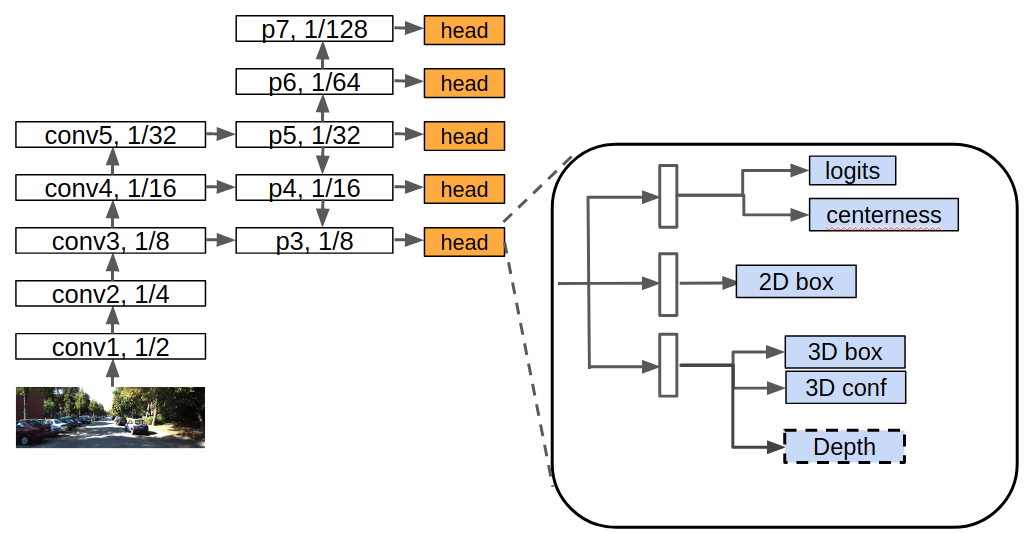
\includegraphics[width=1.0\columnwidth]{figures/fcos3d_arch.png}
	\caption{FCOS-3D extends FCOS to perform 3D detection and dense depth prediction. As in FCOS, a shared head is applied to all levels of FPN features, but with one exception: the depth head is only applied on to the highest resolution features (i.e. $\texttt{p3}$ features).}
\end{figure}

\begin{itemize}
    \item FCOS3D extends FCOS to predict 3D bounding box, in addition to category labels and 2D bounding box.
    \item The output of 3D box head consists of projected centroid, depth of centroid, and size of the 3D box.
    \item Backbone: DLA-34
    \item Matching: Given a 2D bounding box of a foreground object, we associate the features that are within $R$ pixels from the center of 2D bounding box with the given instance.
    \item Loss function: We use disentangled 3D box loss introduced in MonoDis.
    \item 3D confidence: As in MonoDis, we use the 3D confidence, predicted by an additional head, to reweight the logit-based classification score
\end{itemize}

\subsection{Depth pretraining for FCOS-3D}
Dataset: IODA dataset consist of 3.4M pairs or image and Lidar pointcloud. The dataset covers diverse urban environment across US and Japan. The pointcloud is captured by high-resolution Luminar device.
\begin{itemize}
    \item We extend FCOS-3D to perform dense prediction task by aggregating the output of conv2D layer of 3D box head. That is, we upsample all low-resolution features, and add them to produce a dense (stride=4) feature map, and compute depth estimation.
    \item Loss function: we investigate various loss functions, and conclude L1-loss works best. 
    \item Range-aware pretraining. The most challenging instances in monocular 3D detection are in 20-40m range. Therefore, we investigate whether focusing on this range of depth in pretraining helps.
    \item Scale law: We investigate how much of image-pointcloud pairs are needed for a good transfer.
\end{itemize}
\subsection{Depth fine-tuning for FCOS-3D}
\begin{itemize}
    \item Once pretrained, we fine-tune FCOS-3D in multi-task framework, using KITTI3D dataset.
    \item We project Lidar points onto image plane, and use the same archiecture for pretraining to predict sparse per-pixel depth, in addition to the original FCOS-3D losses.
\end{itemize}


\subsection{Pseudo-Lidar 3D detection}
\label{subsec:pseudo-lidar}
PL methods consist of two stages: first, leveraging dense depth estimators, a point cloud is computed given an input RGB image; second, a 3D detector consumes the generated point cloud, outputting detections. The modularity of the PL pipeline implies that any depth estimation method can easily be combined with any detector that consumed point cloud data as input. Moreover, this paradigm allows easy introspection of both components, permitting us to quantify how changes in one affects performance in the other. 

\subsubsection{Monocular depth estimation}
\label{subsubsec:monodepth}

The aim of monocular depth estimation is the recovery of a function $f_D: I \to D$ that predicts for each pixel $p \in I$ the estimated depth $\hat{D} = f_D\left( I\left(p\right)\right)$. Given ground truth depth measurement $D$ (typically acquired by an external sensor, e.g. a LiDAR or RGB-D camera), we define a loss aimed at minimizing the error between the predicted and the actually depth. Formally, our depth estimation model $f_D$ and parameterized by $\theta_D$ is defined as $\hat{\theta}_D = \argmin_{\theta_D}\mathcal{L}_{D}\left(D,\hat{D}\right)$. In all our experiments we 

% \begin{equation} \label{eq:supervised_depth}
% 
% \end{equation}


We supervise our predictions using the scale invariant error proposed by~\cite{eigen2014depth}:  

\begin{equation} \label{eq:silog_loss}
\small
\mathcal{L_D}(D, \hat{D}) =
\frac{1}{N} \sum_{d \in D} e ^2 - \frac{\lambda}{N^2} \left(\sum_{d \in D} e \right)^2
\end{equation}

\noindent where $e$ denotes the error in log space between the predicted and actual depth, $e = \log \hat{d} - \log d$. We follow~\cite{lee2019big} and set $\lambda=0.85$ in all our experiments. We experiment with the PackNet~\cite{guizilini20203d} state-of-the-art network architectures: (i) which uses packing and unpacking blocks with 3D convolutions, allowing it to recover fine structures with high precision; and (ii) BTS~\cite{lee2019big} which leverages local planar guidance layers at different levels allowing better correlation between encoded features and desired output depth  for all our experiments we use the \textit{densenet161} backbone.

% Formally, our depth estimation model $f_D$ and parameterized by $\theta_D$ is defined as: 

% \begin{equation} \label{eq:supervised_depth}
% \hat{\theta}_D = \argmin_{\theta_D}\mathcal{L}_{D}\left(D,\hat{D}\right)
% \end{equation}

% \noindent{\textbf{Loss function.}} We supervise our predictions using the scale invariant error proposed by~\cite{eigen2014depth}:  

% follow~\cite{eigen2014depth} and supervise our predictions using the scale-invariant loss 

% through the Scale Invariant Logarithmic Loss function (SILog) defined as:

% error in log space $\Delta d = \log d - \log \hat{d}$:
% \begin{equation} \label{eq:silog_loss}
% \small
% \mathcal{L_D}(D, \hat{D}) =
% \frac{1}{N} \sum_{d \in D} e ^2 - \frac{\lambda}{N^2} \left(\sum_{d \in D} e \right)^2
% \end{equation}

% \noindent where $e$ denotes the error in log space between the predicted and actual depth, $e = \log \hat{d} - \log d$. We follow~\cite{lee2019big} and set $\lambda=0.85$ in all our experiments.

% \noindent{\textbf{Network architecture.}} We experiment with two state-of-the-art network architectures: (i) PackNet~\cite{guizilini20203d} which uses packing and unpacking blocks with 3D convolutions, allowing it to recover fine structures with high precision; and (ii) BTS~\cite{lee2019big} which leverages local planar guidance layers at different levels allowing better correlation between encoded features and desired output depth  for all our experiments we use the \textit{densenet161} backbone.

% this is particularly relevant for PL methods~\cite{ma2020rethinking,simonelli2020demystifying,qi2018frustum} that leverage an off-the-shelf 2D detector, and perform 3D detection only on image patches where objects have been detected. 

% \noindent{\textbf{Guided training.}} Supervised training of depth estimation network applies the same amount of weight to all supervision points. However, we primarily interested in recovering depth on objects, with depth on other surfaces being less relevant. We follow standard PL~\cite{ma2020rethinking,simonelli2020demystifying,qi2018frustum} practices and assume the availability of an off-the-shelf 2D detector, which we use to detector regions of interest (i.e. objects) in the images. Inspired by keypoint regression methods, we define a mask around object centers, denoted by $\mathcal{M}_{obj}$. We use a Gaussian kernel to associate a weight with each pixel depending on its distance from the object center (see Fig.~\ref{fig:object_masks}). 

% \begin{figure}[h!]
% 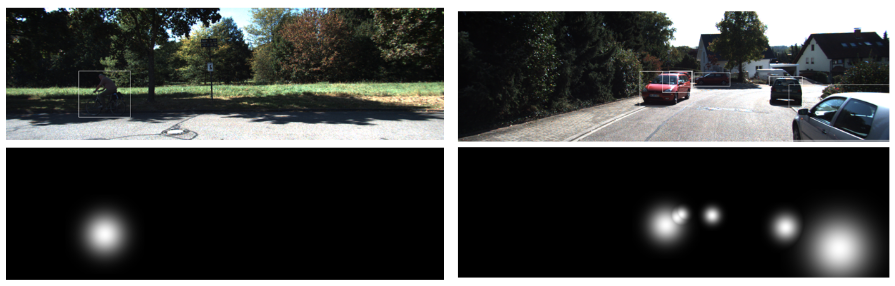
\includegraphics[width=\columnwidth]{figures/object_masks.png}
% \caption{\textbf{Proposed guiding masks for supervised monocular depth training.}}
% \label{fig:object_masks}
% \end{figure}

% We leverage the object masks while training the depth estimation network, and adjust our supervision loss to:

% \begin{equation} \label{eq:masked_silog_loss}
% \small
% \mathcal{L_{MD}}(D, \hat{D}) = \mathcal{L_D}(D, \hat{D}) \circ \mathcal{M}_{obj}
% \end{equation}

% \noindent where $\circ$ to denotes element-wise multiplication. We show in our experiments that the proposed depth guided training scheme improves depth in crucial image regions, leading to improved 3D object detection. 

% \noindent{\textbf{Dataset bias.}} PL methods leverage monocular 3D detectors trained in the same domain. Overlaps in training / validation splits between the two tasks may lead to corrupted results. In the case of the KITTI~\cite{geiger2012we} dataset, the \textit{Eigen train/val} splits proposed in~\cite{eigen2014depth} and commonly used for supervised depth  training~\cite{packnet-semisup,lee2019big,fu2018deep}, overlap with the training and validation set of the KITTI 3D dataset, as described in~\cite{simonelli2020demystifying}. Following~\cite{simonelli2020demystifying}, we remove all overlapping images and generate a new split which we refer to as \textit{Eigen clean}. This procedure is described in more detail in Sec.~\ref{sec:experiments} as well as the supplementary; we will make the new split public to facilitate the generation of unbiased results. We mention that \textit{the depth used by our PL 3D detectors is always trained on Eigen clean, and not on Eigen train}, to avoid any contamination. 



\subsubsection{3D detection}
\label{subsubsec:pl_3d_det}

Our Pseudo-Lidar monocular 3D detector follows the method proposed by~\cite{qi2018frustum,ma2020rethinking}. Given an input image $I$, we predict dense per pixel depth which is converted to a point cloud using the camera intrinsics $K$. For each image pixel $p \in I$ and predicted depth $\hat{d}$, we compute associated 3D point $P$ through: $P=K^{-1}\left[p_x, p_y, \hat{d}\right]$. The point cloud is concatenated with the input image, resulting in a 6D tensor encompassing pixel color values along with 3D coordinates. Leveraging an off-the-shelf 2D detector, proposal regions are identified in images and are fed to a 3D detection network that outputs bounding box parameters. 

\noindent{\textbf{Backbone, detection head and 3D confidence.}}
We follow~\cite{ma2020rethinking}, and process each RoI with a ResNet-18~\cite{he2016deep} backbone that uses Squeeze-and-Excitation layers~\cite{hu2018squeeze}. As the RoI contains both object as well as background pixels, the resulting features are filtered via a foreground/background mask computed based on the associated RoI depth map~\cite{ma2019accurate}. The detection head follows~\cite{ma2020rethinking} and operates in 3 distance ranges, outputting one bounding box for each range; the final output is then selected based on the mean depth of the input RoI. Following~\cite{simonelli2019disentangling,simonelli2020demystifying}, we modify the detection head and also output a 3D confidence value $\gamma$ per detection, which is linked to the 3D detection loss (the architectural details are described in the supplementary).

\noindent{\textbf{Loss function.}} Following~\cite{qi2018frustum} the 3D regression loss is defined as:

\begin{equation} \label{eq:3D_bbox_loss}
\small
\mathcal{L}_{3D} = \mathcal{L}_{center} +  \mathcal{L}_{size} +  \mathcal{L}_{heading} +  \mathcal{L}_{corners}
\end{equation}

We define an additional loss that links the predicted 3D confidence $\gamma$ with the 3D box coordinates loss~\cite{simonelli2019disentangling} using a Binary Cross Entropy (BCE) formulation with target $\hat{\gamma}=e^{-\mathcal{L}_{corners}}$. The final PL 3D detection loss is:

\begin{equation} \label{eq:3D_bbox_loss}
\small
\mathcal{L}_{PL} = \mathcal{L}_{3D} +  \mathcal{L}_{conf}
\end{equation}


\section{Experimental settings}
\label{sec:experiments}


\subsection{Datasets}

\noindent\textbf{KITTI3D~\cite{geiger2012we}.} KITTI 3D detection dataset consists of $7481$ images used for training, and $7518$ images used as the official \emph{test} set. We follow the standard protocol of further splitting the training set into $3712$ and $3769$ images \cite{}, and denote them by \emph{train} and \emph{val}, respectively. We perform all ablative analysis in Sec.~\ref{ablative}  by training on \emph{train} set and evaluating on \emph{val} set. The standard metrics of KITTI benchmark consist of per-class average precision (\emph{AP}) computed with thresholds on intersection-over-union (\emph{IoU}) of 3D boxes and Bird-Eye-View (2D) boxes. In order to evaluate multiclass detectors in Sec.~\ref{ablative}, we additionally use mean average precision (\emph{mAP}) by computing the average of per-class APs, as in recently introduced datasets \cite{caesar2020nuscenes, gahlert2020cityscapes}.  When reporting results on the benchmark, we train on combined set of \emph{train} and \emph{val}, and perform cross-validation with 80/20 splits.

\noindent\textbf{KITTI-depth~\cite{geiger2013vision}.} We report depth estimation results on the standard KITTI depth estimation benchmark. We follow the training protocol of Eigen et al.~\cite{eigen2014depth}, i.e. the KITTI Eiten train and test splits containing $22600$ and $697$ test images. For a fair comparison with the current state-of-the-art~\cite{ma2019accurate,fu2018deep} we report our metrics by comparing against the improved groudtruth LiDAR depth maps introduced in~\cite{geiger2013vision}. As described in Sec~\ref{subsubsec:monodepth}, we generate a new split by removing Eigen train images that overlap (spatially within 50 meters) with the KITTI3D images; we denote this split by \textit{Eigen clean} and mention that for 3D detection the depth networks are finetuned on Eigen clean and \textbf{not on} Eigen train, as has been the standard practice until recently~\cite{simonelli2020demystifying}. We thus avoid contaminating our detection results due to the depth networks overfitting on KITTI3D train/val and exhibiting poor generalization to KITTI3D test. We demonstrate the difference in 3D detection metrics when using Eigen train vs Eigen clean for depth training in the supplementary.

\noindent\textbf{CityScapes3D~\cite{gahlert2020cityscapes}.} CityScapes 3D consists of $5000$ images of urban scenes, split into $2975$ images for training, $500$ for validating, and $1525$ for testing. It is tailored for monocular 3D detection, in that the ground-truth 3D bounding box annotations are obtained using stereo imagery, and therefore avoids annotation artifacts due to parallax and synchronization error with respect to the Lidar sensor. The detection benchmark requires to report 3D bounding boxes of 6 vehicle types. The evaluation metric, \emph{mean detection score} (\emph{mDS}), is computed as the average four depth-dependent metrics measuring errors in predicted center distance, orientation, and size, weighted by 2D detection metric (\emph{AP}).

\noindent\textbf{nuScenes~\cite{caesar2020nuscenes}.} nuScenes dataset consists of $1000$ multimodal videos with full $360$-degree field of view, capturing urban areas of Boston and Singapore from 6 cameras and Lidar / Radar devices. The videos are split into $700$ videos for training, $150$ for validating, and $150$ for testing. The 3D detection benchmark requires to report 3D bounding boxes of 10 object classes over 2Hz-sampled video frames of 360-degree view. The evaluation metric, \emph{nuScenes detection score} (\emph{NDS}), is computed by combining detection accuracy (\emph{mAP}) computed over four different thresholds on center distance with five true-positive metrics. Among them, we only consider three metrics that concerns 3D detection, i.e. \emph{ATE}, \emph{ASE}, and \emph{AOE}.

\noindent\textbf{Depth pretraining.} To pretrain our models, we build a large-scale internal dataset that contains monocular videos and accurate ground-truth depth captured from high-resolution Lidar devices across a full 360-degree field of view. It pictures urban scenes in various cities of US and Japan. We randomly subsample $1K$, $5K$, $10K$, and $25K$ videos (10 seconds each), and refer to these datasets as \textbf{Pretrain-[1k, 5k, 10k, 25k]}, respectively.

\subsection{Implementation}
\label{implementation}
\noindent\textbf{Depth pretraining.} 

\noindent\textbf{Pseudo-Lidar.}

\noindent\textbf{FCOS-3D.}

%\subsection{Depth estimation.}
 

%\noindent\textbf{Pretraining.}
%To quantify the effect of depth quality we pretrain our depth estimation networks on a large internal dataset consisting of image and LiDAR pairs. The complete dataset consists of 25K scenes, each scene being captured with a frequency of $10Hz$ over $10$ seconds, for a total of 25M image + LiDAR pairs. We randomly subsample 1K, 5K and 10K scenes from the complete scene set, and generate a total of 4 pretraining splits (including the complete dataset); for brevity, we will refer to these splits as \textbf{1K}, \textbf{5K}, \textbf{10K} and \textbf{25K} whenever appropriate. Importantly, the downsampled splits contain fewer images as well as less diversity, as we downsample from the scene set and not from the image set. We use the generated splits for pre-training the depth networks, and we perform experiments that estimate depth quality vs. 3D detection performance at each pretraining level. We describe the pretraining protocol in detail in the supplementary. 

% and mention that we ensured that each model is trained to convergence. 


% \subsection{FCOS-3D}
% \textbf{Pretraining backbone}
% \begin{figure}[t]
% 	\centering
% 	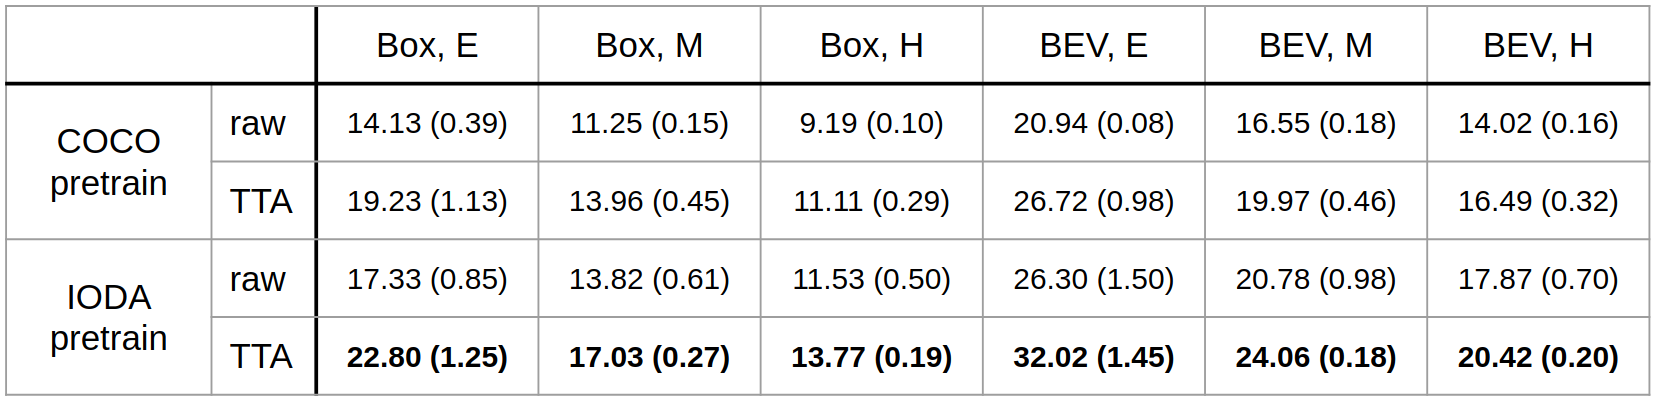
\includegraphics[width=1.0\columnwidth]{figures/fcos3d_backbone_pretrained.png}
% \end{figure}


\section{Analysis and results}
\label{sec:results}
We present detailed analysis on our pretraining and finetuning strategy, as well as benchmark results of our two proposed detectors on three 3D detection benchmarks.




\begin{figure}[h]
    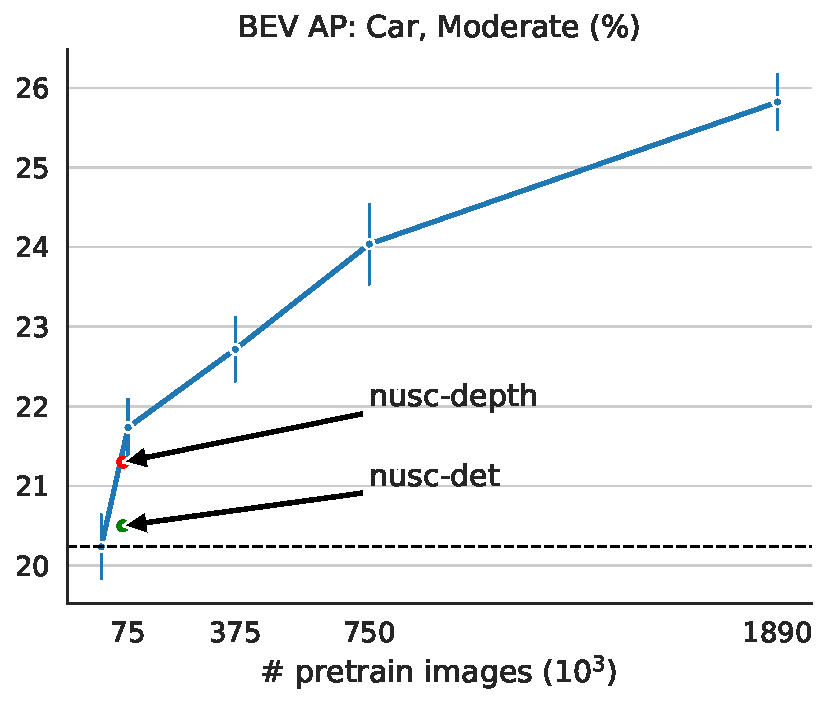
\includegraphics[width=0.99\columnwidth,trim={0mm 0mm 0mm 0mm},clip]{figures/scaling_law.pdf}
    \caption{Accuracy of 3D detection continues to improve, at least up to 1.89M images used for pre-training. We pre-train FCOS-3D with growing sizes of image-pointcloud pairs until convergence. The models are then fine-tuned on for 3D detection on KITTI \emph{train}, and evaluated on KITTI \emph{val}.}
    \label{fig:pretraining_vs_depth}
\end{figure}


\begin{table}[t!]
\centering
{
\footnotesize
\setlength{\tabcolsep}{0.4em}
\rowcolors{2}{lightgray}{white}
\begin{tabular}{l|ccc|ccc}
\toprule
& \multicolumn{3}{c}{BEV AP} & \multicolumn{3}{c}{3D AP} \\ 
\multirow{-2}{*}{Pre-train task}& 
Car & 
Pedestrian &
Cyclist &
Car & Pedestrian & Cyclist \vspace{0.5mm}\\
\midrule
%  DLA-34, Det2D & 
% 16.84 & 
% 7.01 &
% 2.88 &
% 11.20 &
% 5.64 &
% 2.40
% \\
2D-det (coco)  & 
% 16.84 & 
% 7.01 &
% 2.88 &
% 11.20 &
% 5.64 &
% 2.40
20.24 & 
7.82 &
3.77 &
13.94 &
6.01 &
3.13
\\
\midrule
% DLA-34, Depth & 
% 21.70 & 
% 9.29 &
% 3.30 &
% 15 .06 &
% 7.33 &
% 2.75
% \\
+ 2D-det (nusc) & 
x.xx & 
x.xx &
x.xx &
x.xx &
x.xx &
x.xx
\\
+ Depth  (nusc) & 
x.xx & 
x.xx &
x.xx &
x.xx &
x.xx &
x.xx
\\
\midrule
+ Depth (internal) & 
\textbf{25.82} & 
\textbf{9.93} &
\textbf{4.36} &
\textbf{18.20} &
\textbf{7.64} &
\textbf{3.75}
\\
\bottomrule
\end{tabular}\\\vspace{0mm}
\caption{We aim to ablate the role of pre-training on depth estimation via controlled experiments. We use FCOS-3D to pre-train subset of parameters relevant to each pre-train task, and fine-tine on KITTI \emph{train} for 3D detection. \textbf{2D-det} denotes 2D bounding box detection as pre-training task; \textbf{Depth} denotes supervised depth prediction using ground-truth depth available from Lidar point-cloud. Starting from parameters pre-trained on MS-COCO dataset (2D detection), we perform additional pre-training in target domain (i.e. autonomous driving) on either 2D detection or depth estimation, using the \emph{same} set of images (\textbf{nusc}) until convergence. To understand how the accuracy scales with respect to the size of pre-train data, we internally collect a large set of image-Lidar pairs (\textbf{internal}) and use it for depth pre-training. The fine-tuned models are evaluated on KITTI \emph{val}. We only report "Moderate" metrics. Depth pretraining significantly improves 3D detection accuracy, up to \textbf{30.6\%} from the baseline pre-training method.}
\label{table:dla-34}
}
\end{table}

\begin{table}[t!]
\centering
{
\footnotesize
\setlength{\tabcolsep}{0.4em}
\rowcolors{2}{lightgray}{white}
\begin{tabular}{c|ccc|ccc}
\toprule
& \multicolumn{3}{c}{BEV AP} & \multicolumn{3}{c}{3D AP} \\ 
\multirow{-2}{*}{Pre-train task}& 
Car & 
Pedestrian &
Cyclist &
Car & Pedestrian & Cyclist \vspace{0.5mm}\\
\midrule
%  DLA-34, Det2D & 
% 16.84 & 
% 7.01 &
% 2.88 &
% 11.20 &
% 5.64 &
% 2.40
% \\
2D Det. (coco)  & 
8.40 & 
2.49 &
0.09 &
4.58 &
1.70 &
0.03
\\
% \midrule
% DLA-34, Depth & 
% 21.70 & 
% 9.29 &
% 3.30 &
% 15 .06 &
% 7.33 &
% 2.75
% \\
% 2D Det. (coco + nuim) & 
%x.xx & 
%x.xx &
%x.xx &
%x.xx &
%x.xx &
%x.xx
%\\
%Depth & 
%x.xx & 
%x.xx &
%x.xx &
%x.xx &
%x.xx &
%x.xx
%\\
  + Depth & 
\textbf{24.27} & 
\textbf{9.59} &
\textbf{3.34} &
\textbf{17.34} &
\textbf{8.17} &
\textbf{2.65}
\\
\bottomrule
\end{tabular}\\\vspace{0mm}
\caption{Pre-training on supervised depth estimation allows for training larger backbone of FCOS-3D. We pre-train V2-99 \cite{lee2019centermask} backbone (96.9M parameters) using 2D detection on MS-COCO dataset, and perform additional pre-training using depth prediction on our internal dataset of image-pointcloud pairs. The models are then fine-tuned on KITTI \emph{train} for 3D detection, and evaluated on KITTI \emph{val}. The depth pre-training significantly improve rare classes: 4$\times$ for "Pedestrian", 37$\times$ for "Cyclist". We run each fine-tuning experiment four times, and report the average. We only report "Moderate" metrics due to limited space.}
\label{table:v2-99}
}
\end{table}

\subsection{3D detection}
\label{subsec:3d_detection}

\noindent\textbf{KITTI3D} Our numbers on the \textit{validation split} of the KITTI3D dataset are summarized in Table~\ref{table:kitti_3d_val} for the BEV and 3D detection tasks. We note that our baseline numbers are on par with related methods, and we record a significant increase in performance when using the modifications proposed in this paper. Our baseline FCOS-3D model uses COCO~\cite{lin2014microsoft} pretraining and we record an increase of $22\%$ by using depth estimation as an auxiliary task for pretraining ($17.03$ vs $13.96$). Our PL numbers improve over the current state-of-the-art on this split by $58\%$ and over our baseline by $75\%$ ($22.31$ vs $14.10$ and $12.68$ respectively). Note that we are omitting from this comparison the results reported by methods that use depth trained on images that overlap with the KITTI3D train and val splits. 

% , as discussed in detail in Sec.~\ref{subsec:eigen_clean}, e.g.~\cite{weng2019monocular,ma2019accurate,ding2020learning}.

Our numbers on the \textit{test split} of the KITTI3D dataset are reported in Table~\ref{table:kitti_3d_test}. Our novel single-stage 3D detector (\textit{FCOS-3D}) outperforms all other single and two-stage detectors, with a notable improvement of $21\%$ over the previous best published results for the Car - Easy category (i.e. in 3DAP $20.09$ vs. $15.54$); our improvements are significantly more noticeable on smaller classes (i.e. cyclists and pedestrians), as reported in the supplementary. Our PL-based detector also outperforms the previous state-of-the-art in this category by a significant margin - for Car - medium our 3DAP is $11\%$ higher (i.e. $13.05$ vs $11.72$). We ablate the various components of our method in Sec.~\ref{subsec:ablative_analysis}.


\begin{table}[t!]
\centering
{
\footnotesize
\setlength{\tabcolsep}{0.4em}
\rowcolors{2}{lightgray}{white}
\begin{tabular}{l|ccc|ccc}
\toprule
& \multicolumn{3}{c}{BEV AP} & \multicolumn{3}{c}{3D AP} \\ 
\multirow{-2}{*}{Depth net}& 
Easy & 
Med &
Hard &
Easy & Med & Hard \vspace{0.5mm}\\
\midrule
% ROI-10D~\cite{manhardt2019roi} & 
% 9.78 & 
% 4.91 &
% 3.74 &
% 4.32 &
% 2.02 &
% 1.46
% \\
% GS3D~\cite{li2019gs3d} & 
% 8.41 & 
% 6.08 &
% 4.94 &
% 4.47 &
% 2.90 &
% 2.47
% \\
MonoGRNet~\cite{qin2019monogrnet} & 
19.72 & 
12.81 &
10.15 &
11.90 &
7.56 &
5.76
\\

% MonoPSR~\cite{ku2019monocular} & 
% 18.33 & 
% 12.58 &
% 9.91 &
% 10.76 &
% 7.25 &
% 5.85
% \\

% SS3D~\cite{jorgensen2019monocular} & 
% 16.33 & 
% 11.52 &
% 9.93 &
% 10.78 &
% 7.68 &
% 6.51
% \\

MonoDIS (single)~\cite{simonelli2019disentangling} & 
18.45 & 
12.58 &
10.66 &
11.06 &
7.60 &
6.37
\\

M3D-RPN~\cite{brazil2019m3d} & 
20.85 & 
15.62 &
11.88 &
14.53 &
11.07 &
8.65
\\

% SMOKE~\cite{liu2020smoke} & 
% 20.83 & 
% 14.49 &
% 12.75 &
% 14.03 &
% 9.76 &
% 7.84
% \\

MonoPair~\cite{chen2020monopair} & 
24.12 & 
18.17 &
15.76 &
16.28 &
12.30 &
10.42
\\

MonoDIS (multi)~\cite{simonelli2020disentangling} & 
23.40 & 
17.20 &
15.30 &
16.50 &
12.20 &
10.30
\\

Kinematic3D~\cite{brazil2020kinematic} & 
27.83 & 
19.72 &
15.10 &
19.76 &
14.10 &
10.47
\\

\midrule

Baseline: FCOS-3D & 
%26.72 &
%19.97 &
%16.49 &
%19.23 &
%13.96 &
%11.11 
26.77 &
20.24 &
16.72 &
18.84 &
13.94 &
11.25 
\\

Ours: FCOS-3D & 
% 32.02 &
% 24.06 &
% 20.42 &
% 22.80 &
% 17.03 &
% 13.77
33.23 &
25.82 &
21.75 &
24.01 &
18.20 &
14.85
\\


% Baseline: BTS + PL & 
% 31.90 &
% 22.14 &
% 19.24 &
% 22.75 &
% 15.61 &
% 13.34 
% \\


\midrule
Baseline: PL &  % PackNet 
25.42 &	
17.97 &	
15.22 &  
18.50 & 
12.68 & 
10.78
\\


Ours: PL &  % PackNet 
\textbf{43.46} & 
\textbf{29.96} &
\textbf{25.07} &
\textbf{34.01} &
\textbf{22.31} &
\textbf{18.58} 
\\

% Ours: BTS + PL & 
% 31.90 &
% 22.14 &
% 19.24 &
% 22.75 &
% 15.61 &
% 13.34 
% \\



\bottomrule
\end{tabular}\\\vspace{0mm}
\caption{
\textbf{3D detection performance on the KITTI3D validation set} for the Car category using the AP$|_{R_{40}}$ metric.}
\label{table:kitti_3d_val}
}
\end{table}


\begin{table}[t!]
\centering
{
\footnotesize
\setlength{\tabcolsep}{0.4em}
\rowcolors{2}{lightgray}{white}
\begin{tabular}{l|ccc|ccc}
\toprule
& \multicolumn{3}{c}{BEV AP} & \multicolumn{3}{c}{3D AP} \\ 
\multirow{-2}{*}{Depth net}& 
Easy & 
Med &
Hard &
Easy & Med & Hard \vspace{0.5mm}\\
\midrule
ROI-10D~\cite{manhardt2019roi} & 
9.78 & 
4.91 &
3.74 &
4.32 &
2.02 &
1.46
\\
GS3D~\cite{li2019gs3d} & 
8.41 & 
6.08 &
4.94 &
4.47 &
2.90 &
2.47
\\
MonoGRNet~\cite{qin2019monogrnet} & 
18.19 & 
11.17 &
8.73 &
9.61 &
5.74 &
4.25
\\
MonoPSR~\cite{ku2019monocular} & 
18.33 & 
12.58 &
9.91 &
10.76 &
7.25 &
5.85
\\

SS3D~\cite{jorgensen2019monocular} & 
16.33 & 
11.52 &
9.93 &
10.78 &
7.68 &
6.51
\\

MonoDIS (single)~\cite{simonelli2019disentangling} & 
17.23 & 
13.19 &
11.12 &
10.37 &
7.94 &
6.40
\\

M3D-RPN~\cite{brazil2019m3d} & 
21.02 & 
13.67 &
10.23 &
14.76 &
9.71 &
7.42
\\

SMOKE~\cite{liu2020smoke} & 
20.83 & 
14.49 &
12.75 &
14.03 &
9.76 &
7.84
\\

MonoPair~\cite{chen2020monopair} & 
19.28 & 
14.83 &
12.89 &
13.04 &
9.99 &
8.65
\\



Kinematic3D~\cite{brazil2020kinematic} & 
26.99 & 
17.52 &
13.10 &
19.07 &
12.72 &
9.17
\\

MonoDIS (multi)~\cite{simonelli2020disentangling} & 
24.45 & 
19.25 &
16.87 &
16.54 &
12.97 &
11.04
\\




Ours FCOS-3D & 
%\textbf{29.03} & 
%\textbf{19.63} &
%\textbf{16.78} &
%\textbf{20.09} &
%\textbf{13.04} &
%\textbf{11.02}
\textbf{29.41} & 
\textbf{19.59} &
\textbf{16.95} &
\textbf{20.90} &
\textbf{13.48} &
\textbf{11.27}
\\




\midrule


MonoPL$\dagger$~\cite{weng2019monocular} & 
0.0 & 
0.0 &
0.0 &
10.76 &
7.50 &
6.10
\\


AM3D$\dagger$~\cite{ma2019accurate} & 
25.03 & 
17.32 &
14.91 &
16.50 &
10.74 &
9.52
\\


PatchNet$\dagger$ ~\cite{ma2020rethinking} & 
22.97 & 
16.86 &
14.97 &
15.68 &
11.12 &
10.17
\\


\textit{RefinedMPL$\dagger$ ~\cite{vianney2019refinedmpl}} & 
\textit{28.08} & 
\textit{17.60} &
\textit{13.95} &
\textit{18.09} &
\textit{11.14} &
\textit{8.96}
\\


D4LCN$\dagger$~\cite{ding2020learning} & 
22.51 & 
16.02 &
12.55 &
16.65 &
11.72 &
9.51
\\

\textit{Demystifying$\dagger$~\cite{simonelli2020demystifying}} & 
\textit{-} & 
\textit{-} &
\textit{-} &
\textit{23.66} &
\textit{13.25} &
\textit{11.23}
\\


Ours PL & 
\textbf{28.87} & 
\textbf{18.57} &
\textbf{15.74} &
\textbf{20.78} &
\textbf{13.05} &
\textbf{10.66}
\\


\bottomrule
\end{tabular}\\\vspace{0mm}
\caption{
\textbf{3D detection performance on the KITTI3D test set} for the Car category using the AP$|_{R_{40}}$ metric. $\dagger$ denotes pseudo-lidar based methods.}
\label{table:kitti_3d_test}
}
\end{table}

\begin{table}[t!]
\centering
{
\footnotesize
\setlength{\tabcolsep}{0.4em}
\rowcolors{2}{lightgray}{white}
\begin{tabular}{l|ccc|ccc}
\toprule
& \multicolumn{3}{c}{Pedestrian} & \multicolumn{3}{c}{Cyclist} \\ 
\multirow{-2}{*}{Methods}& 
Easy & 
Med &
Hard &
Easy & Med & Hard \vspace{0.5mm}\\
\midrule
OFTNet~\cite{} &
1.28 &
0.81 &
0.51 &
0.36 &
0.16 &
0.15 
\\
SS3D~\cite{} &
2.48 &
2.09 &
1.61 &
3.45 &
1.89 &
1.44 
\\
M3D-RPN~\cite{} &
5.65 &
4.05 &
3.29 &
1.25 &
0.81 &
0.78 
\\
MonoPSR~\cite{} &
7.24 &
4.56 &
4.11 &
\textbf{9.87} &
\textbf{5.78} &
\textbf{4.57} 
\\
MonoDIS (multi)~\cite{simonelli2020disentangling} & 
9.07 & 
5.81 &
5.09 &
1.47 &
0.85 &
0.61
\\
\midrule
FCOS-3D & 
\textbf{15.86} & 
\textbf{10.49} &
\textbf{9.06} &
5.00 &
3.06 &
2.56
\\
\bottomrule
\end{tabular}\\\vspace{0mm}
\caption{
Multiclass 3D detection on KITTI3D test set. We report BEV AP$|_{R_{40}}$ metrics for "Pedestrian" and "Cyclist" category. FCOS-3D outperforms most of other approaches, with \textbf{80.5\%} improvement from the previous best method on "Pedestrian".}
\label{table:kitti_3d_test_multi_class}
}
\end{table}

\subsection{Depth estimation}
\label{subsec:depth_estimation}


\begin{table}[t!]
\renewcommand{\arraystretch}{1.00}
\centering
{
\small
\setlength{\tabcolsep}{0.4em}
\rowcolors{2}{lightgray}{white}
\begin{tabular}{l|cccc}
\toprule
% \multirow{2}{*}{\textbf{Method}} &
% \multicolumn{3}{|c|}{Lower is better $\downarrow$} &
% \multicolumn{3}{|c}{Higher is better $\uparrow$} \\
Method & 
Abs.Rel$\downarrow$ &
Sqr.Rel$\downarrow$ &
RMSE$\downarrow$ &
$\delta_{1.25}\uparrow$ 
% a2 &
% a3
\\
\toprule

Kuznietsov et al. \cite{kuznietsov2017semi}
% & 0.113 & 0.741 & 4.621 & 0.862 & 0.960 & 0.986
& 0.113 & 0.741 & 4.621 & 0.862 
\\
Gan et al. \cite{Gan2018MonocularDE}
% & 0.098 & 0.666 & 3.933 & 0.890 & 0.964 & 0.985
& 0.098 & 0.666 & 3.933 & 0.890
\\
Guizilini et al. ~\cite{packnet-semisup}
% & 0.078 & 0.378 & 3.330 & 0.927 & --- & ---
& 0.078 & 0.378 & 3.330 & 0.927 
\\
Fu et al. \cite{fu2018deep}
% & 0.072 & 0.307 & 2.727 & 0.932 & 0.984 & 0.994
& 0.072 & 0.307 & 2.727 & 0.932
\\
Yin et al. \cite{Yin2019enforcing}
% & 0.072 & --- & 3.258 & 0.938 & 0.990 & 0.998
& 0.072 & --- & 3.258 & 0.938 
\\
Lee et al. ~\cite{lee2019big} 
% & 0.059 & 0.245 & 2.756 & 0.956 & 0.993 & 0.998
& 0.059 & 0.245 & 2.756 & 0.956
\\

\midrule

Ours PackNet 
% & 0.053 & 0.179 & 2.301 & 0.968 & 0.996 & 0.999
& 0.053 & 0.179 & 2.301 & 0.968
\\
Ours BTS
% & 0.051 & 0.166 & 2.234 & 0.972 & 0.996 & 0.999
& 0.051 & 0.166 & 2.234 & 0.972
\\

\bottomrule

\end{tabular}
}
\caption{\textbf{Depth estimation results on the KITTI dataset}, for the \textit{Eigen} test split \cite{eigen2014depth} and distances up to 80m.} 
\label{table:depth_kitti}

\end{table}



\noindent{\textbf{KITTI.}} To better quantify the performance of our depth estimation component as well as place is within context, we perform experiments on the standard monocular depth estimation benchmark using the KITTI dataset. We report results with both the PackNet and BTS network architectures: we first pre-train on the $25K$ image split, and subsequently fine-tune on the Eigen train split; we report results on the Eigen test split. The exact training protocol is described in detail in the supplementary. Our results are summarized in Table~\ref{table:depth_kitti}. We compare against the current state-of-the-art and note that while other methods use ImageNet pretraining, our depth pretraining significantly improves performance by up to $30\%$ for some metrics ($0.166$ vs $0.245$ \textit{Sqr.Rel}). Our numbers indicate the our monocular depth results outperform all other published methods to date by a large margin. 

\subsection{A critical analysis of depth estimation metrics}
\label{subsec:depth_metrics}

\subsection{The impact of data on depth and 3D detection}
\label{subsec:depth_pretraining}

\begin{figure*}[t!]
% \vspace{-1mm}
\centering

\subfloat{
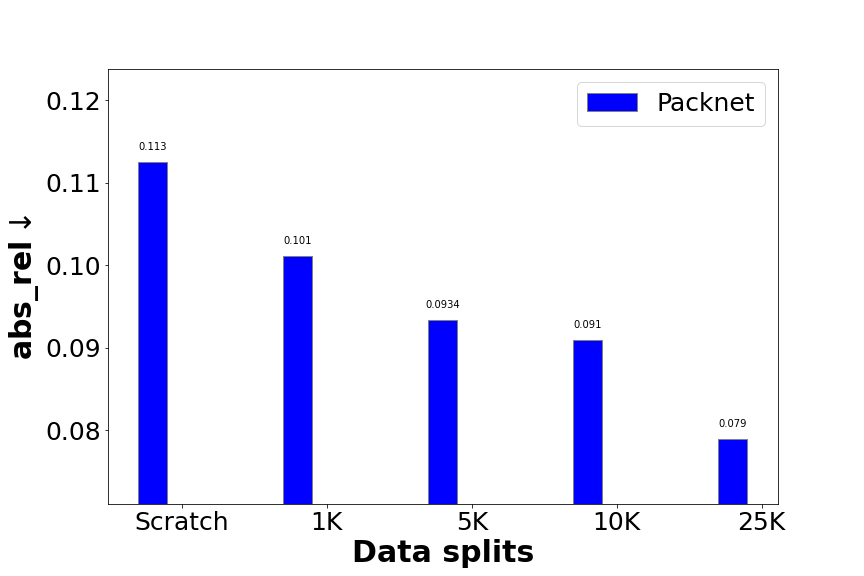
\includegraphics[width=0.3\linewidth]{figures/scaling_laws/PacknetFT_depth_metrics_k3d_val_abs_rel.png}
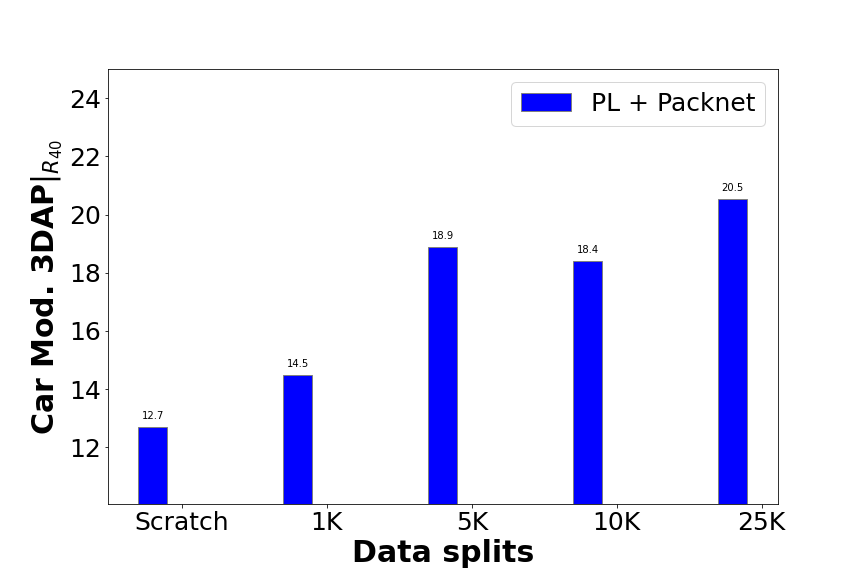
\includegraphics[width=0.3\linewidth]{figures/scaling_laws/Packnet_3d_det.png}
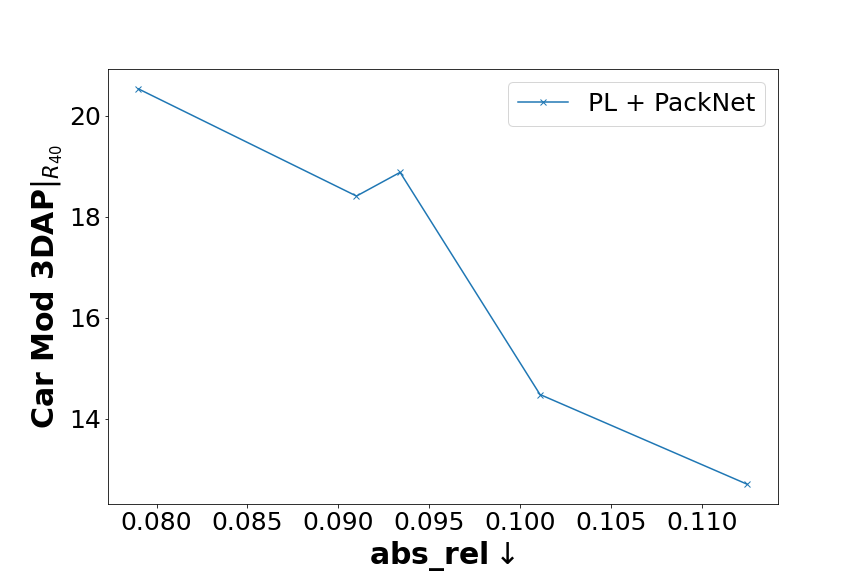
\includegraphics[width=0.3\linewidth]{figures/scaling_laws/depth_vs_3d_det_AP_3d_metrics_Mod.png}
}
\caption{
\textbf{Depth quality vs 3D AP for varying dataset sizes.} \textbf{Left:} we report the proposed \textit{abs\_rel} per-object depth metric on the KITTI3D validation split; the depth network is pretrained with varying dataset sizes and fine-tuned on the KITTI Eigen-clean split. \textbf{Middle:} for each depth network, a PL 3D detector is trained on KITTI 3D train and evaluated on KITTI 3D val. \textbf{Right:} we plot the proposed abs\_rel metric vs the resulting 3D AP metric; note that both are computed on the KITTI 3D validation split.
}
\label{fig:scaling_laws_packnet}
\end{figure*}

% -------------------------------------------------
% \begin{figure}[h]
%     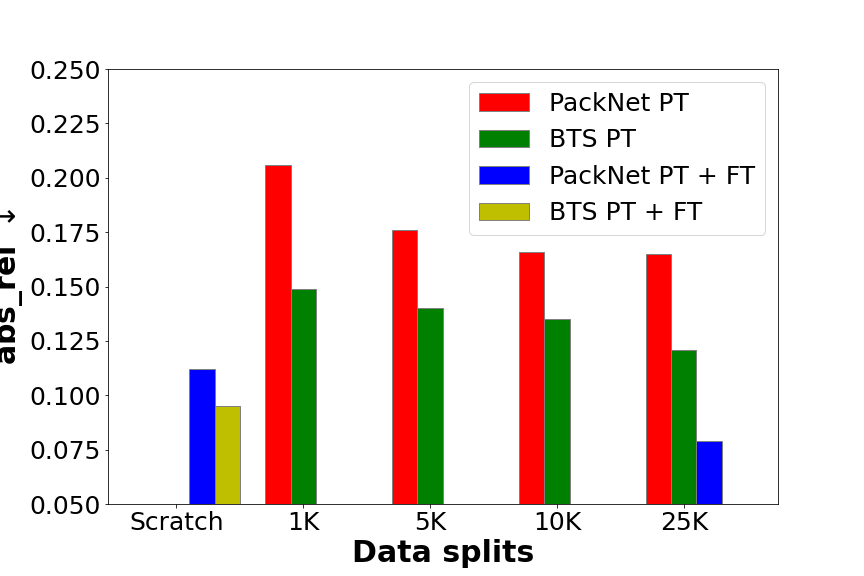
\includegraphics[width=0.99\columnwidth,trim={0mm 0mm 0mm 0mm},clip]{figures/depth_ft_transfer.png}
%     \caption{\textbf{Depth metrics on the KITTI3D validation set}: we report results for the $abs\_rel$ metric for the PackNet and BTS architectures after pre-training on varying dataset sizes. \textbf{PT} denotes pure transfer after pretraining, while \textbf{PT + FT} denotes pretraining and fine-tuning on the KITTI Eigen clean split.}
%     \label{fig:pretraining_vs_depth}
% \end{figure}

% \begin{figure}[h]
%     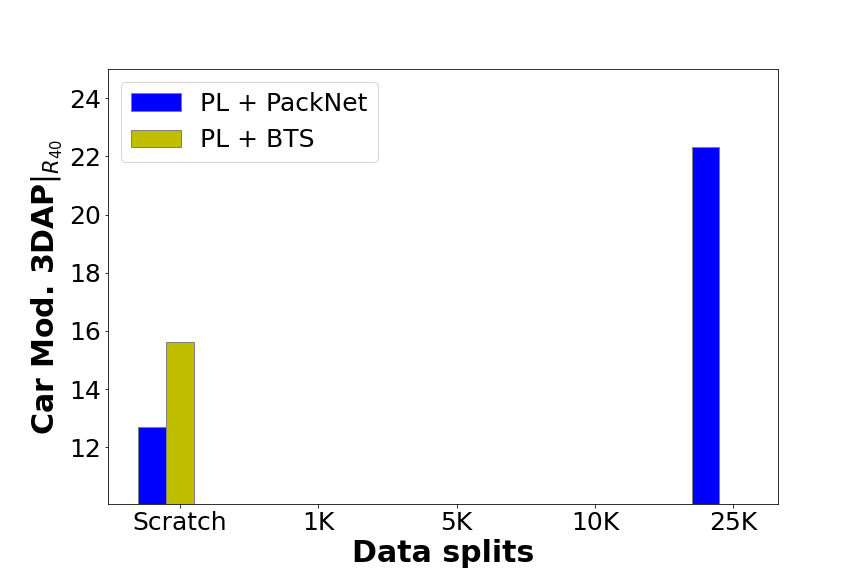
\includegraphics[width=0.99\columnwidth,trim={0mm 0mm 0mm 0mm},clip]{figures/pretraining_3d_det.png}
%     \caption{\textbf{Moderate Car 3D AP results on the KITTI validation set for the PL and FCOS3D detectors.} The depth networks are pretrained on varying dataset sizes and fine-tuned on the KITTI Eigen clean split.}
%     \label{fig:pretraining_vs_3D_det}
% \end{figure}

\subsection{Ablative analysis}
\label{subsec:ablative_analysis}


\begin{table}[t!]
\centering
{
\footnotesize
\setlength{\tabcolsep}{0.4em}
\rowcolors{2}{lightgray}{white}
\begin{tabular}{l|ccc|ccc}
\toprule
& \multicolumn{3}{c}{BEV AP} & \multicolumn{3}{c}{3D AP} \\ 
\multirow{-2}{*}{Depth net}& 
Easy & 
Med &
Hard &
Easy & Med & Hard \vspace{0.5mm}\\
\midrule
PackNet & 
41.59 & 
27.75 &
23.69 &
30.91 &
20.53 &
17.25
\\
PackNet + 2D masks  & 
40.46 & 
27.64 & 
23.03 &
32.39 &
21.29 & 
17.97 
\\

PackNet + Gauss. masks &
43.46 &
29.96 &
25.07 &
34.01 &
22.31 &
18.58 
\\



\bottomrule
\end{tabular}\\\vspace{0mm}
\caption{
\textbf{Ablative analysis of 3D detection performance with different depth fine-tuning strategies.}}
\label{table:baseline_depth_detection}
}
\end{table}







\section{Conclusion}
\input{sections/conclusion}

{\small
\bibliographystyle{ieee_fullname}
\bibliography{egbib}
}

\end{document}
